\subsection{Multipleksere}
\label{Multipleksere}
%
Multiplekserens formål er at agere kontaktfunktion mellem de enkelte filtre. Kontaktfunktionen kan vælger én af to forskellige inputspændinger og levere den valgte spænding på udgangen. På den måde er det ved hjælp af multiplekseren muligt at til- eller fravælge de enkelte filtre. Multiplekserens formål er derudover at agere kontaktfunktion mellem rækken af forstærkende og dæmpende filtre, afhængigt af komparatorens output. På den måde er det muligt at vælge om de lave frekvenser i signalet, der sendes videre til effektforstærkeren, skal være dæmpet eller forstærket. Multiplekserens kontaktfunktioner skal kunne skifte stadie på baggrund af et digitalt binært input, fra A/D konverteren.\\[5mm]
%
Til formålet vælges en tredobbelt 2-kanals analog multiplekser, nærmere bestemt HEF4053B, hvis datablad fremgår af \textcite{PDF:Multiplekser}. At det er en 2-kanals multiplekser betyder at den har en kontaktfunktion, som kan vælge én af to inputs og levere det som output. At den er tredobbelt betyder at der sidder tre 2-kanals kontaktfunktioner i det integrede kredsløb. Det er, ved at benytte en enkelt HEF4053B multiplekser, muligt at til- eller fravælge tre filtre. Dette er i midlertid ikke nok for at til- eller fravælge samtlige enkelte filtre. Der benyttes derfor tre multipleksere af typen HEF4053B, for at nok kontaktfunktioner er tilgængelige mellem filtrene. De tre multipleksere bidrager tilsammen med ni kontaktfunktioner, hvoraf kun syv bruges til at skifte mellem de enkelte filtre. En af de overskydende kontakter anvendes derfor til at agere kontaktfunktion mellem rækken af forstærkende og dæmpende filtre, hvis stadie afhænger af komparatorens output. Der er derfor kun en enkelt overskydende kontakt.
%
\begin{figure}[H]
	\centering
	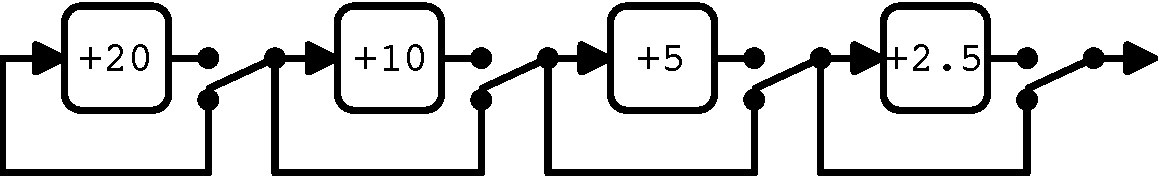
\includegraphics[resolution=300,scale=\circuitSize]{Figure/Circuits/Multiplekser.pdf}
	\caption{Illustration af hvordan multiplekseren kobles til filtrene.}
	\label{fig:Multiplekser}
\end{figure}
\noindent
%
På \autoref{fig:Multiplekser} illustreres det hvordan kontaktfunktionen enten kan være i et stadie der aktiverer et filter eller i et stadie hvor signalet passerer uden om filteret. Afhængigt af hvordan kontakterne står, er det muligt at aktivere flere filtre for en større forstærkning. 
 
Multiplekserens kontakter skifter stadie på baggrund af et digitalt binært input. Inputtet leveres på multiplekserens tre inputterminlaer: S1, S2 og S3, hvor hver inputterminal styrer hver deres respektive kontaktfunktion: 1Z, 2Z og 3Z. Leveres et digitalt lavt input på S1, indstilles kontaktfunktionen til stadiet 1Y0, hvorfor spændingen på 1Y0 inputterminalen sendes videre til 1Z outputterminalen. Leveres der i stedet et digitalt højt input på S1, indstilles kontaktfunktionen til stadiet 1Y1 og spændingen på 1Y1 inputterminalen sendes videre til 1Z outputterminalen.\\                    
